%!TEX root = ../../thesis.tex

\section{Data-Driven Model}
\label{sec:Data_Driven_Model}
We identify a difference equation for the temperature evolution with semiparametric regression, using 51 weeks of experimental data collected from the fourth floor of SDH. Semiparametric regression in buildings has been proposed by \cite{Aswani:2012aa}, where the authors used only one week of historic data to model the temperature evolution and used the HVAC's supply air temperature as the single control input. % including an exogenous heating load that captures the effect of occupancy, electric devices, outside air temperature, and solar radiation. 
We extend this approach by taking into account multiple weeks, which we separate into three seasons (fall, winter, spring) so as to characterize the different levels of the exogenous heating load for different temporal seasons. 
In addition, we model the room temperatures as a function of airflow rates from multiple VAVs to obtain a model which can be used for more sophisticated control strategies.
%We make use of cross-validation across all weeks to find the optimal model, therefore allowing for a more general analysis of the thermal behavior rather than restricting ourselves to identifying a model tailored to a single week, as is done in \cite{Aswani:2012aa}.

Next, we first introduce the semiparametric method using a simple lumped zone model of the fourth floor, and then identify a multi-zone model for the same floor which we will use to make quantitative comparisons with the physics-based model.

\subsection{Lumped Zone}
\label{sec:Lumped_Zone}
\subsubsection{Model Setup}
In order to facilitate analysis, the entire 4th floor of SDH is treated as a single zone, with the scalar temperature $x$ corresponding to the %area-averaged zone 
average temperature on the entire floor and the input $u$ as the sum of the inflow of all 21 VAV boxes. %This lumped model assumes a uniform temperature on the entire floor, $x$, and has been commonly used in literature \cite{Ma:2012aa, Oldewurtel:2010aa}. 
Then, the temperature evolution is assumed to have the following form:
\begin{equation}\label{eq:Temperature_evolution}
x(k+1) = a x(k) + b u(k) + c^\top v(k) + q_{\text{IG}}(k) + \epsilon(k),
\end{equation}
where %$u$ denotes the total air inflow to the entire floor and 
$v := \left[v_\text{Ta}, v_\text{Ts}, v_\text{solE}, v_\text{solN}, v_\text{solS}, v_\text{solW} \right]^\top$ is a vector of known disturbances that describes ambient air temperature, the HVAC system's supply air temperature, and solar radiation from each of the four geographical directions.
In addition, $q_{\text{IG}}$ represents the internal gains due to occupancy and electric devices, and $\epsilon$ denotes independent and identically distributed zero mean noise with constant and finite variance which is conditionally independent of $x$, $u$, $v$, and $q_{\text{IG}}$. Finally, $a$, $b \in \mathbb{R}$ and $c \in \mathbb{R}^6$ are unknown coefficients to be estimated using semiparametric regression \cite{Ruppert:2003aa, Hardle:2000aa}.

\subsubsection{Smoothing of Time Series}
The $q_{\text{IG}}$ term of Equation \eqref{eq:Temperature_evolution} is treated as a nonparametric term, so that \eqref{eq:Temperature_evolution} becomes a partially linear model. By taking conditional expectations on both sides of \eqref{eq:Temperature_evolution}, we obtain

\begin{equation}\label{eq:Conditional_Expectation}
\begin{aligned}
\hat{x}(k+1) &= a\hat{x}(k) + b\hat{u}(k) + c^\top\hat{v}(k) \\
& \quad + \mathbb{E}\left[ q_{\text{IG}}(k) \vert k \right] + \mathbb{E}\left[ \epsilon(k) \vert k \right],\\
\end{aligned}
\end{equation}
\noindent
where the conditional expectations $\hat{x}(\cdot) = \mathbb{E}\left[ x(\cdot) \vert \cdot \right]$, $\hat{u}(\cdot) = \mathbb{E}\left[ u(\cdot) \vert \cdot \right]$, and $\hat{v}(\cdot) = \mathbb{E}\left[ v(\cdot) \vert \cdot \right]$ are used.
Noting that $\mathbb{E}\left[ \epsilon(\cdot) \vert \cdot \right] = 0$ and assuming $\mathbb{E}\left[ q_{\text{IG}}(\cdot) \vert \cdot \right] = q_{\text{IG}}(\cdot)$, subtracting \eqref{eq:Conditional_Expectation} from \eqref{eq:Temperature_evolution} gives
\begin{equation}\label{eq:subtract}
\begin{split}
x(k+1) - \hat{x}(k+1) = a\left( x(k) - \hat{x}(k) \right) \\ + b\left( u(k) - \hat{u}(k) \right)
+ c^\top \left( v(k) - \hat{v}(k) \right) + \epsilon(k).
\end{split}
\end{equation}
The unknown internal gains term has been eliminated, and thus the coefficients $a, b, c$ in \eqref{eq:subtract} can be estimated with any regression method.

The conditional expectations $\hat{x}(\cdot), \hat{u}(\cdot)$ and $\hat{v}(\cdot)$ are obtained by smoothing the respective time series \cite{Aswani:2012aa}. We made use of locally weighted linear regression with a tricube weight function, where we use $k$-fold cross-validation to determine the bandwidth for regression.
%that assigns weights $\psi_i$ 
%\begin{equation}\label{eq:tricube_weight_function}
%\psi_i = \left( 1- \left| \frac{z-z_i}{d(z)} \right|^3 \right)^3, 
%\end{equation}
%that belong to $z_i \in \mathcal{Z}$, which is a neighbor of the data point $z$ to be smoothed along the abscissa within the span $\mathcal{Z}$ (all data points around $z$ taken into account to smooth the time series at $z$), and $d(z)$ the distance from $z$ to the farthest predictor within $\mathcal{Z}$. The width $d(z)$ of the span $\mathcal{Z}$ is determined with $k$-fold cross-validation.
The error measure used for in-sample estimates is the \textit{Root Mean Squared} (RMS) \textit{Error} between the measured temperatures $\bar{x}(k)$ and the model's predicted temperatures $x(k)$ over a time horizon of $N$ steps (e.g. we chose a 24 hour time horizon, $N = 96$):
\begin{equation}\label{eq:RMS}
\text{RMS error} = \left(\frac{1}{N}\textstyle\sum_{k=1}^N \left[\bar{x}(k) - x(k)\right]^2 \right)^{1/2}.
\end{equation}
\subsubsection{Bayesian Constrained Least Squares}
A main challenge in identifying the model is that commercial buildings are often insufficiently excited. Take SDH for example, whose room temperatures under regular operation only vary within a range of 2$^{\circ}$C and inflow of the VAV boxes hardly varies at all. To overcome this, data collected during forced response experiments described in Section \ref{sec:exp_data} was used in training the model. To further compensate for the lack of excitation, a Bayesian regression method is used, which allows our prior knowledge of the building physics to be incorporated in the identification of coefficients. More specifically, Gaussian prior distributions are used for the coefficients $a$ and $b$, i.e., $a \sim \mathcal{N}( \mu_a, \Sigma_a)$ and $b \sim \mathcal{N}( \mu_b, \Sigma_b)$, where $\mathcal{N}( \mu, \Sigma)$ denotes a jointly Gaussian distribution with mean $\mu$ and covariance matrix $\Sigma$. In addition, $a$, $b$ and $c$ are constrained to be identical for the different seasons, since they model the underlying physics of the building which are assumed to be invariant throughout the year. 

Let $\mathcal{T} = \{1, 2, \cdots, N\}$ denote the $N$ weeks of training data (e.g. we chose $N = 45$), and define $\mathcal{F} = \{i \in \mathcal{T} \text{ such that $i$ is a week in fall} \}$ as the set of training weeks from the fall season. Similarly, define the sets of training weeks from the winter and spring as $\mathcal{W}$ and $\mathcal{S}$.
The coefficient identification problem is then formulated as follows:
\begin{equation}\label{eq:data_opt}
\begin{aligned}
(\hat{a}, \hat{b} , \hat{c}) = &\arg\min_{a, b, c}~\left(J_\mathcal{F} + J_\mathcal{W} + J_\mathcal{S}\right) + \Vert \Sigma_a^{-1/2} (a - \mu_a) \Vert^2\\
& \quad\quad + \Vert \Sigma_b^{-1/2} (b - \mu_b)  \Vert^2 \\
\text{s.t.}~ J_\mathcal{X}= & \textstyle \sum_{i \in \mathcal{X}} \Vert x_i(k+1) - \hat{x}_i(k+1) - a\left( x_i(k) - \hat{x}_i(k) \right)\\
& - b\left( u_i(k) - \hat{u}_i(k) \right) - {c}^\top\left( v_i(k) - \hat{v}_i(k) \right) \Vert ^ 2\\
& \text{for } \mathcal{X} \in \lbrace \mathcal{F}, \mathcal{W}, \mathcal{S} \rbrace, \\
& 0 < a < 1,~ b \leq 0,~ c \geq 0. \\
\end{aligned}
\end{equation}
%where subscripts f, w, and s represent fall, winter and spring, respectively. 
In other words, $J_\mathcal{F}$, $J_\mathcal{W}$ and $J_\mathcal{S}$ represent the sum of squared errors between experimentally measured temperatures and model's predicted temperatures for fall, winter and spring, respectively.
The sign constraints on the parameters $b$ and $c$ translate into the fact that the temperature to be estimated positively correlates with all components in $v$ and negatively correlates with the VAV airflow. The range of $a$ is a consequence of Newton's Law of Cooling.
%One problematic aspect that greatly complicates the identification of the coefficients is the little excitation of the system, since the observed temperatures vary within a small range only (e.g. 20-22$^{\circ}$C for fall and spring weeks, and 19-21$^{\circ}$C for the winter weeks) and the inflow of the single VAV boxes hardly vary at all. Contrary to \cite{Aswani:2012aa}, where the authors used Bayesian Linear Regression, which relies on covariance matrices penalizing regularization terms and which are set in a subjective fashion, we use a grid search algorithm coupled with Least Squares approximation to determine the optimal set of parameters $(\hat{a}, \hat{b}, \mathbf{\hat{c}})$ that minimize the sum of the weekly RMS of the individual seasons \eqref{eq:RMS}, with the constraint that $(\hat{a}, \hat{b})$ are identical for the different seasons since it is assumed that the inherent physics of the lumped zone remain unchanged throughout the year. We therefore formulate the problem as follows:
%\begin{equation}\label{eq:grid_search}
%\begin{aligned}
%& \hat{a}, \hat{b} = \arg\min_{a, b}~\left(\text{RMS}_f + \text{RMS}_w + \text{RMS}_s\right) \\
%& \text{s.t.}~\hat{c}_j = \arg\min_{c_j} \Vert T_j(n+1) - \hat{T}_j(n+1) - a\left( T_j(n) - \hat{T}_j(n) \right)\\
%& - b\left( u_j(n) - \hat{u}_j(n) \right) - c_j\left( w_j(n) - \hat{w}_j(n) \right) \Vert
% \\
%& j \in \lbrace\text{fall}, \text{winter}, \text{spring}\rbrace
%\end{aligned}
%\end{equation}
%That is, for a fixed pair of coefficients $(a, b)$, $\mathbf{\hat{c}}_j$ is defined to be the minimizer of the described loss function for season $j$ which we determine with Least Squares fitting. The optimal parameters $\hat{a}, \hat{b}, \mathbf{\hat{c}}$ are therefore the triplet of parameters that minimize the sum of the RMS over all seasons.\\
%Figure \ref{fig:RMS_seasons} shows the RMS for the individual seasons and the mean for different parameters $\left(a, b\right)$ to solve \eqref{eq:grid_search}. It can be seen that the heat maps for the three different seasons exhibit different characteristics. For fall and spring, the optimal value of $a$ appears to be $\approx 0.85$, whereas the RMS in winter period decreases beyond $a>0.85$. The RMS takes a minimum for $a\approx 0.87, b\approx 0.03$. However, the average RMS heat map indicates that the RMS hardly increases for the given range of parameters $a, b$, since the maximum mean RMS exceeds the optimum by $<10\%$ only.
%\begin{figure}[hbtp]
%\centering
%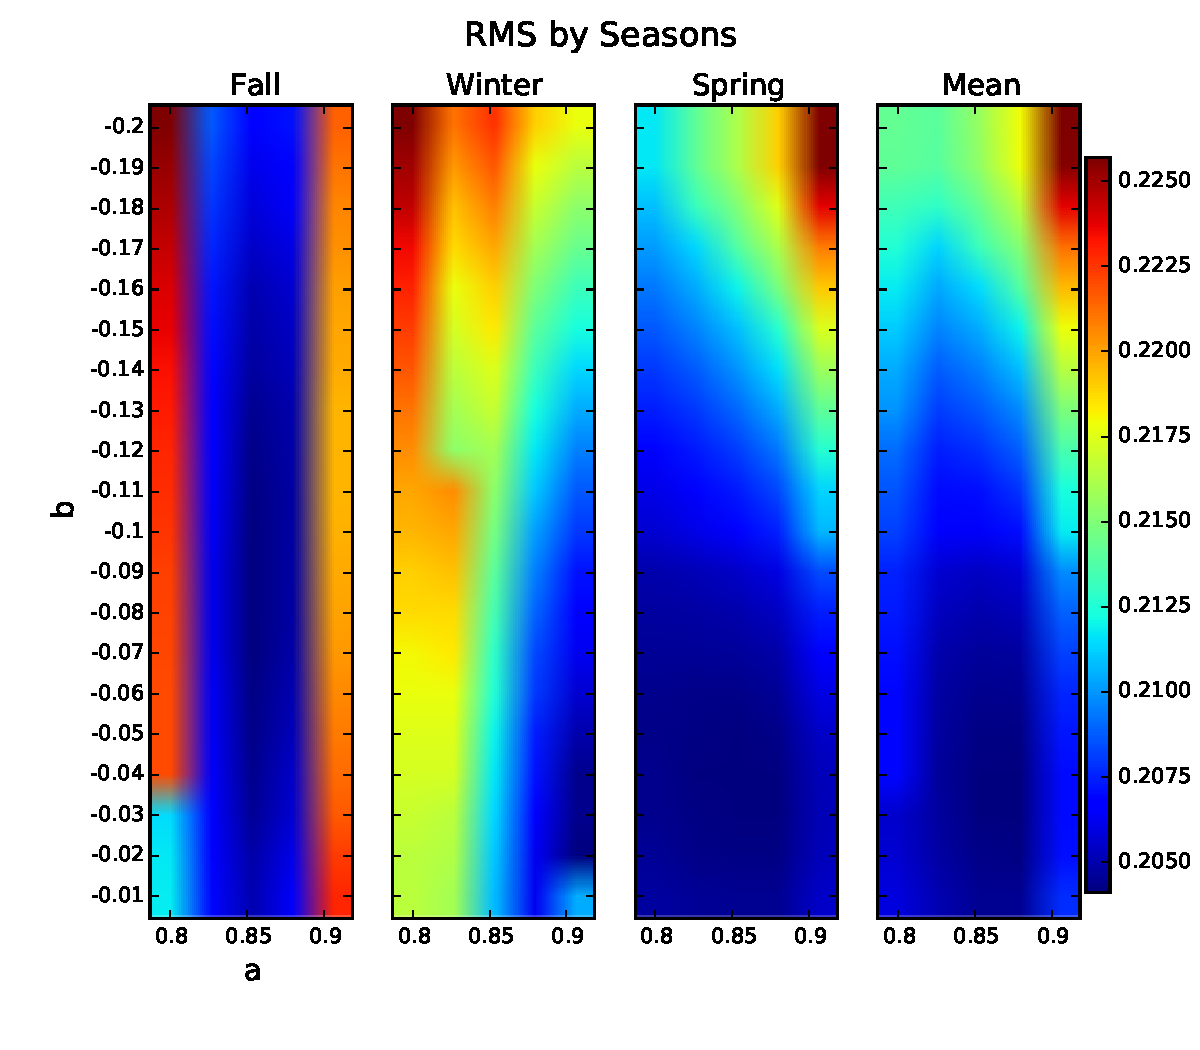
\includegraphics[scale=0.42]{Figures/RMS_cumul.pdf}
%\caption{RMS for different seasons with different $\hat{a}$, $\hat{b}$}
%\label{fig:RMS_seasons}
%\end{figure}
%Without the prior terms, the optimal value $b$ that minimizes the cost function in \eqref{eq:data_opt} is found to be $\approx 0.03$. With the unit of the airflow being $\left[kg/s\right]$, the 15-minute temperature reduction due to an average inflow of $2.2 kg/s$ would only be 0.066$^{\circ}$C.

%Thus, due to the insufficient excitation of the building, we use physical intuition to increase the parameter $b$ from its optimal value $b=0.03$ so as to give the control input more weight without compromising the prediction quality to an unjustifiable extent. 
To find the effect of the VAV inflow on the 15-minute temperature evolution, we computed the 15-minute incremental reductions in temperature $\Delta x$ recorded during the excitation experiments. 
%\footnote{The excitation experiments were carried out on weekends to minimize disruption of building operation. The temperature during these experients were kept within comfort bounds (20-22$^\circ$C).}. 
It is assumed that the large inflow $u$ dominates all other effects such that we can assume
\begin{equation}\label{eq:excitation_equation}
\Delta x = x(k+1) - x(k) = b\cdot u(k)
\end{equation}
for all $k$ during the excitation period. The estimated prior $\mu_b$ can then be isolated from \eqref{eq:excitation_equation}. The prior $\mu_a$ was set as the optimal $\hat{a}$ identified by \eqref{eq:data_opt} without the prior terms. The covariance matrices $\Sigma_a$ and $\Sigma_b$ were chosen subjectively. 
%The result is shown in Figure \ref{fig:decrem_T}. The negative slope of the linear fit corresponds to the prior on $b$. Given this prior $b=-0.18$, we choose the value of $a$ that yields the minimum RMS. Thus, we identify $\hat{a}=0.83, \hat{b} = -0.18$ with a mean RMS of 0.236. 
%\qie{Modify this paragraph to describe choice of prior without figure, and note difference between b value for 1 zone and whole floor, because b depends on the thermal mass of the zone.}
%\begin{figure}[hbtp]
%\centering
%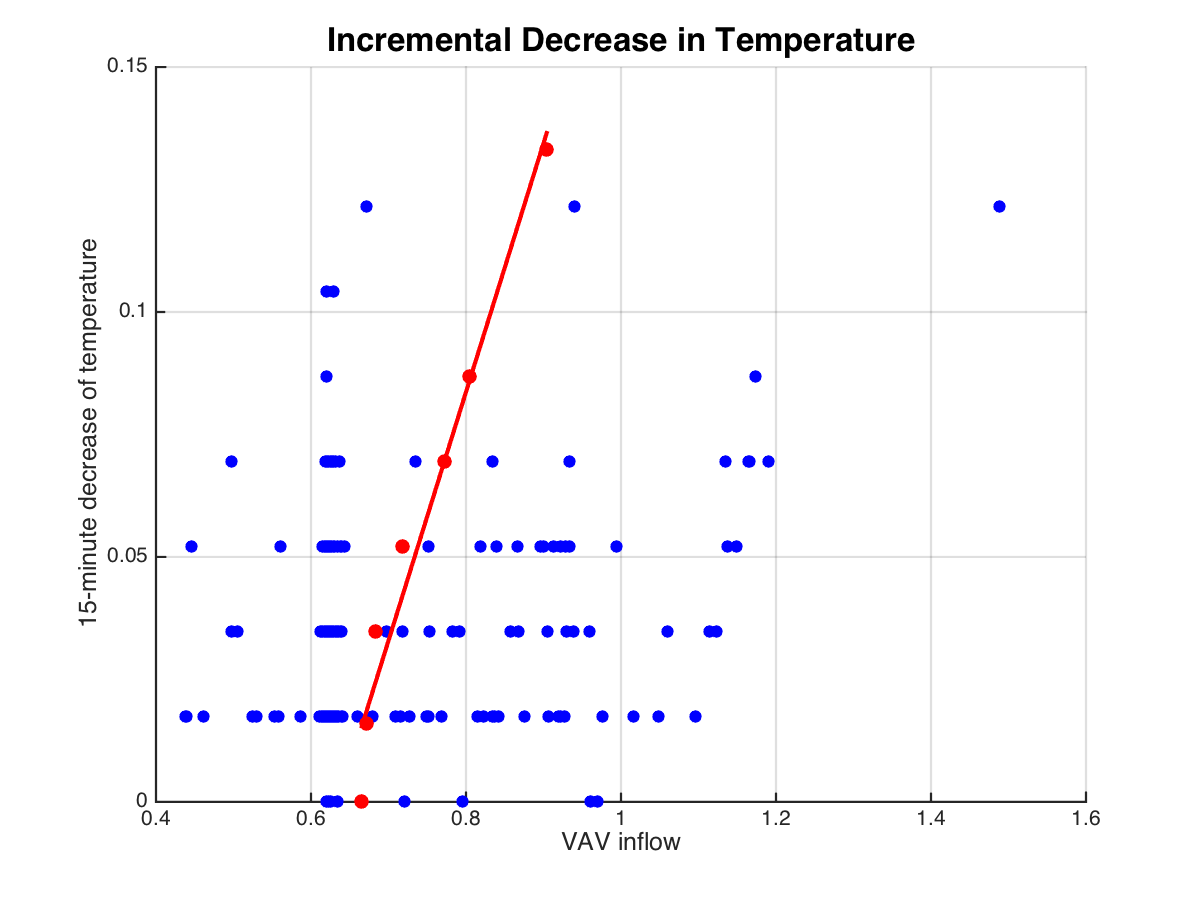
\includegraphics[scale=0.42]{Figures/b_prior.png}
%\caption{Incremental decrease of $T$ due to $u$}
%\label{fig:decrem_T}
%\end{figure}
\subsubsection{Estimation of Internal Gains}
With the estimated coefficients $\hat{a}, \hat{b}, \hat{c}$ in hand, the internal gains $q_{\text{IG}}$ can be estimated by manipulating \eqref{eq:Conditional_Expectation}: 
\begin{equation}\label{eq:qig_estimation}
\hat{q}_{\text{IG}}(k) = \hat{x}(k+1) - \left(\hat{a}\hat{x}(k) + \hat{b}\hat{u}(k) + \hat{c}^\top \hat{v}(k)\right).
\end{equation}
%This can be interpreted as the difference between the smoothed temperature $\hat{x}(k+1)$ and the predicted expected temperature.
%$\mathbb{E}\left[x(k+1)\right]$. \textcolor{red}{(I think this may be what's causing the confusion, because from previous definition $\mathbb{E}\left[x(k+1)\right]$ = $\hat{x}(k+1)$. But this suggests they are different variables. Can we remove this?)} 
%With the estimated parameter coefficients being constant over the different seasons, a distinct function of internal gains is estimated for each season by averaging the estimated weekly gains for a given season.
A distinct function of internal gains is estimated for each season. In other words, \eqref{eq:qig_estimation} is used to estimate an instance of the internal gains function for each week $i$ in the training set $\mathcal{T}$. The internal gains function for each season, $\hat{q}_{\text{IG},\mathcal{X}}$ is then defined as the average of estimated weekly gains for all weeks $i \in \mathcal{X}$ and $\mathcal{X} \in \{ \mathcal{F}, \mathcal{W}, \mathcal{S} \}$.

%From the definition of the temperature model \eqref{eq:Temperature_evolution}, the internal gain at time $k$, overlaid with noise $\epsilon(k)$, could also be estimated as the difference between the measured temperature $\bar{x}(k+1)$ and the predicted temperature $\tilde{x}(k+1)$:
%\begin{equation}\label{eq:qig_observational}
%\hat{q}_{\text{IG}}(k) + \epsilon(k) = \bar{x}(k+1) - \underbrace{\hat{a}\bar{x}(k) - \hat{b}\bar{u}(k) - \hat{c}^\top \bar{v}(k)}_{\tilde{x}(k+1)}.
%\end{equation}

\subsubsection{Results}
The estimated internal gains for each season are shown in Figure \ref{fig:qig_comparison_plot}.
\begin{figure}[hbtp]
\centering
\vspace*{-0.0cm}
\hspace*{-0.6cm}
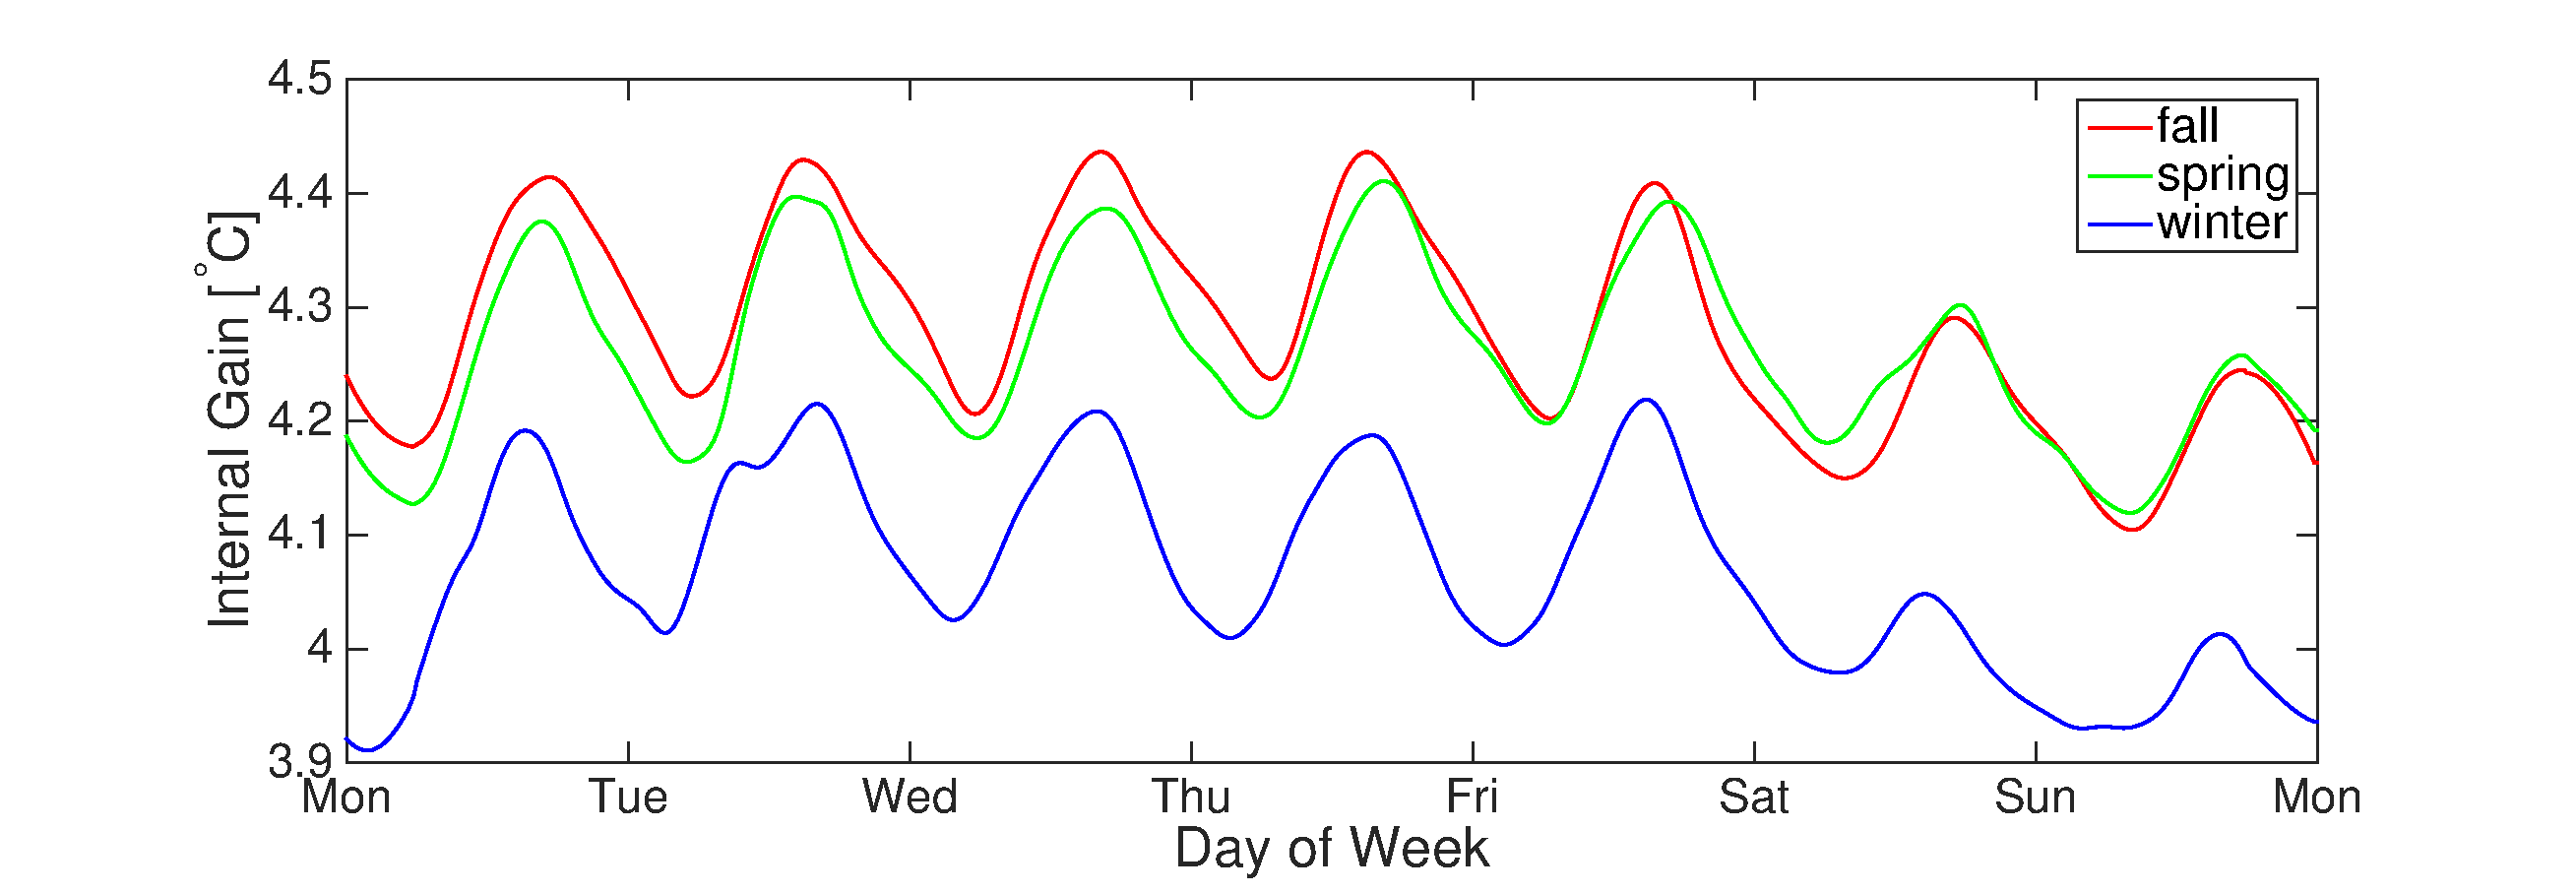
\includegraphics[scale=0.22]{chapters/building_model/figures/data_lump_qig.eps}
\vspace*{-0.3cm}
\caption{Estimated Internal Gain $q_{\text{IG}}$ from the Data-Driven Model by Season, Lumped Case}
\vspace*{-0.3cm}
\label{fig:qig_comparison_plot}
\end{figure}
Observe that, for all three seasons, the internal gains exhibit a daily trend with local peaks around the late afternoon and local minima at night. Moreover, the amplitudes of the internal gains are considerably smaller during the weekends, suggesting a lighter occupancy. It can further be seen that the magnitude of the internal gains is smallest for the winter season, which is in accordance with our intuition since most building occupants are absent during that period.

%Furthermore, computing $q_{\text{IG}}$ with smoothed time series \eqref{eq:qig_estimation} yields smoother results than with \eqref{eq:qig_observational}, since there is no noise term $\epsilon(k)$. This suggests that the difference between the solid and the dashed line represents the zero mean Gaussian noise of \eqref{eq:Temperature_evolution}.

Lastly, since the Bayesian Constrained Least Squares algorithm \eqref{eq:data_opt} has identified a set of parameter estimates $\hat{a}, \hat{b}, \hat{c}$ valid for all three seasons to account for the time-invariant physics of the building, the temperature predictions are of the same nature for all three seasons. We thus conclude that the inherent differences between the seasonal temperature data are captured by the internal gains and can be compared between the seasons on a relative level.

The identified models for the different seasons found with \eqref{eq:data_opt} are
\begin{equation}\label{eq:lumped_zone_res}
\begin{aligned}
x(k+1) & = 0.80\cdot x(k) - 0.18\cdot u(k) \\
 & ~~ + \left[0.0019, 0.028, \mathbf{0} \right] v(k) + q_{\text{IG},\mathcal{X}}(k) \\
 & =  0.80\cdot x(k) - 0.18\cdot u(k) \\
 & ~~ + 0.0019 \cdot v_{\text{Ta}}(k) + 0.028 \cdot v_{\text{Ts}}(k) + q_{\text{IG},\mathcal{X}}(k) \\
 & \text{for } \mathcal{X} \in \lbrace \mathcal{F}, \mathcal{W}, \mathcal{S} \rbrace\\
\end{aligned}
\end{equation}
The estimated coefficients of $c$ corresponding to the solar radiation disturbances are very small ($< 10^{-6}$) compared to the other estimated coefficients. Since the temperatures are of the order $10^{\circ}$C, air inflow around 1 kg/s and solar radiation about 100 W/m$^2$, the effect of solar radiation on the room temperature is orders of magnitude less than that of other factors and hence can be neglected.

The average RMS prediction errors are 0.22$^{\circ}$C, 0.17$^{\circ}$C and 0.23$^{\circ}$C for fall, winter and spring, respectively, showing that our model predicts the temperature reasonably well. 

%Figure \ref{fig:temp_plot_lump} shows a comparison between the actual temperature of the three zones and the predicted temperature with a prediction horizon of $N = 96$ (24 hours) for a selected week of the holdout test data. Note that the predicted temperature is initialized in 24 hour intervals.

%\begin{figure}[hbtp]
%\centering
%\vspace*{-0.31cm}
%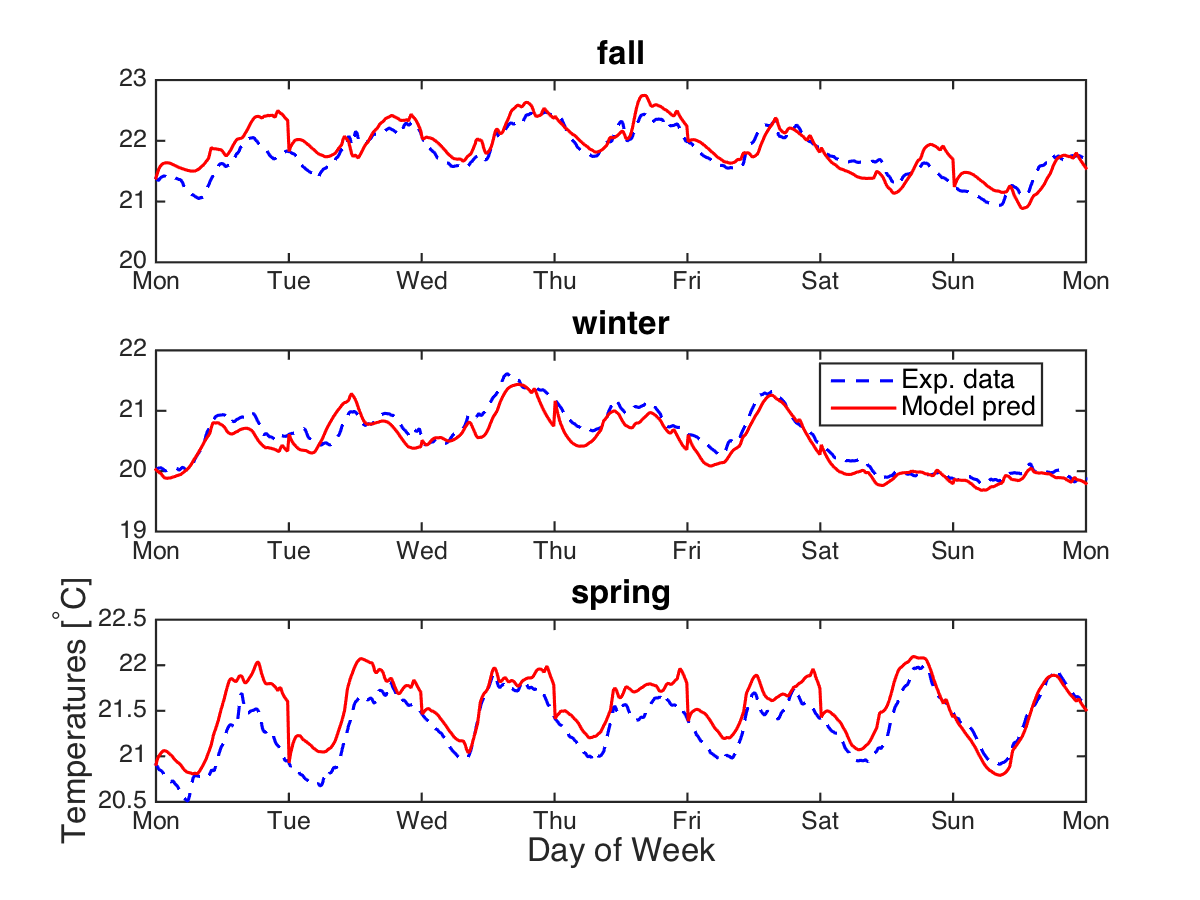
\includegraphics[scale=0.46]{Figures/lumped_test.png}
%\vspace*{-0.7cm}
%\caption{Measured and Predicted Temperatures by Season}
%\label{fig:temp_plot_lump}
%\end{figure}

%Figure \ref{fig:qig_seasons} shows the estimated internal gain for the three seasons fall, winter, and spring identified with \eqref{eq:grid_search} and $\hat{a}=0.83, \hat{b} = -0.18$. 
%\begin{figure}[hbtp]
%\centering
%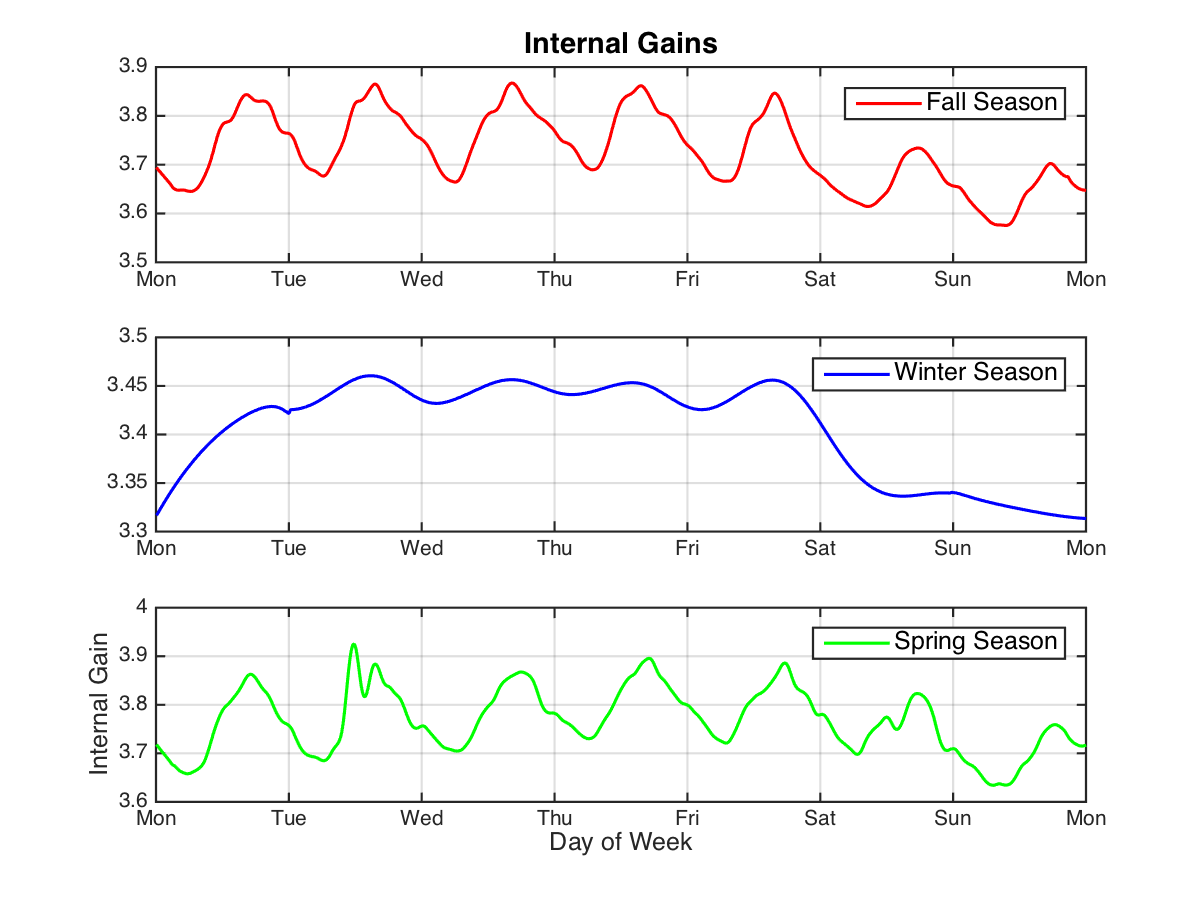
\includegraphics[scale=0.46]{Figures/Internal_gains.png}
%\caption{Estimated internal gains for the seasons, lumped case}
%\label{fig:data_lump_qig}
%\end{figure}
%The models for the different seasons are identified as
%\begin{equation}\label{eq:lumped_zone_res}
%\begin{split}
%T_f(n+1) =& ~0.83\cdot T_f(n) - 0.18\cdot u(n) + \\ &\left[0.0024, 0.0241, \mathbf{0}\right]\cdot w(n) + q_{\text{IG},f}(n) \\
%T_w(n+1) =& ~0.83\cdot T_w(n) - 0.18\cdot u(n) + \\ & \left[0.0185, 0.0186, \mathbf{0}\right]\cdot w(n) + q_{\text{IG},w}(n) \\
%T_s(n+1) =& ~0.83\cdot T_s(n) - 0.18\cdot u(n) + \\ & \left[8\cdot 10^{-10}, 0.0228, \mathbf{0}\right]\cdot w(n) + q_{\text{IG},s}(n)
%\end{split}
%\end{equation}
%In \eqref{eq:lumped_zone_res}, the indices "f", "w", and "s" denote the fall, winter, and spring season, with weekly RMS  0.208, 0.251, 0.250, respectively. The estimated parameters belonging to the known disturbances $w$ are negligible $\left(<1\cdot 10^{-5}\right)$ for the global incidence radiations from the four geographic directions, A possible explanation for these small coefficients could be that the effect of the solar radiation is partially captured by the internal gain $q_{\text{IG}}$. Indeed, we found that the inclusion of a Lasso-regularization term to \eqref{eq:grid_search} shrinks these estimated coefficients $c$ further to zero, with a negligible increase of $q_{\text{IG}}$ and the RMS.\\
%It is important to note that the estimated autoregressive coefficient $\hat{a}$ and the control coefficient $\hat{b}$ have been forced to be identical (equation \eqref{eq:grid_search}), and that the estimated coefficients on the supply air temperature are similar for the three seasons. Further, the estimated coefficient for the outside air temperature has little effect on the temperature evolution. Thus, the only significant difference characterizing seasonal effects is the weekly internal gain, which is shown in Figure \ref{fig:qig_seasons}. The internal gains $q_{\text{IG}}~$ for the different seasons exhibit a daily trend with local peaks around the late afternoon and local minima at night. Moreover, for the fall and spring season, the amplitudes of the internal gain are considerably smaller during the weekend. It can further be seen that the magnitude of the internal gain is smallest for the winter season, which is in accordance with our intuition since most people are absent during that period.\\
\subsection{Individual Zones}\label{sec:Indiv_Zones}
\subsubsection{Model Setup}
Rather than approximating the entire 4th floor of SDH as a single zone, in this section, we identify a multivariate model that describes the thermodynamic behavior of each of the six individual zones:
\begin{equation}
\begin{aligned}\label{eq:temp_propagation_indiv}
x(k+1) &= A x(k) + B u(k) + C v(k) + q_{\text{IG},\mathcal{X}}(k) \\
& ~~ \text{for } \mathcal{X} \in \lbrace \mathcal{F}, \mathcal{W}, \mathcal{S} \rbrace,
\end{aligned}
\end{equation}
where $x$, $q_{\text{IG},\mathcal{X}} \in \mathbb{R}^6$, and the control input $u \in \mathbb{R}^6$ represent the temperatures, the internal gains of each zone, and the total air flow to each zone, respectively. In the lumped case, it was observed that solar radiation only had a negligible effect on the building's thermodynamics compared to the input and other disturbances, and thus we omit the solar radiation in the subsequent analysis: $v := \left[ v_\text{Ta}, v_\text{Ts} \right]^\top \in \mathbb{R}^2$.

Inspired by Newton's Law of Cooling, only adjacent zones influence each other's temperature, which defines the sparsity pattern of the coefficient matrices that are to be estimated. Hence 
\begin{equation}
A_{ij} = \begin{cases}
      \neq 0, & \text{if}\ i=j~\text{or}~(i,j)~ \text{adjacent}  \\
      0, & \text{otherwise.}
    \end{cases}
\end{equation}
The diagonal elements of $A$ denote autoregressive terms for zone temperatures, whereas non-diagonal elements describe the heat exchange between adjacent rooms. The matrix $B$ is diagonal by definition of $u$. The sparsity pattern of $C$ is found by physical adjacency of a respective zone to an exterior wall of a given geographic direction.

\subsubsection{Model Identification}
The procedure for the estimation of the parameter matrices $\hat{A}$, $\hat{B}$, $\hat{C}$, and the internal gains follows \eqref{eq:data_opt}, but with a modified choice of the (now matrix-valued) priors $\mu_a$ and $\mu_b$: $\mu_b$ and the diagonal entries of $\mu_a$ are obtained by scaling the corresponding priors from the lumped zone case in order to account for the thermal masses of the individual zones, which are smaller than in the lumped case. The off-diagonal elements of $\mu_a$, which represent the heat transfer between adjacent zones, were set to a value close to zero, according to our calculations with the heat transfer equation $\dot{q} = U\cdot A \cdot \Delta x$ and \cite{Koehler:2013aa}.
%are approximated with the heat transfer equation
%\begin{equation}
%\dot{q} = U\cdot A \cdot \Delta x,
%\end{equation}
%which describes the heat transfer $\dot{q}$ between two zones with temperature difference $\Delta x$ as a function of the heat transfer coefficient $U$ of the separating wall of area $A$. 
%According to our calculations and \cite{Koehler:2013aa}, the effect is negligible, and thus we set these priors to a value close to zero.
%The grid search algorithm \eqref{eq:grid_search} involves exponential complexity and therefore proves to be computationally intractable in the single zone case because of the large number of states. From a physical point of view, the effect of HVAC cooling and heat evolution for a given zone is identical to the lumped zone case, and thus we fix the diagonal elements of $\mathbf{a}$ to the same value identified for the lumped zone case, $\hat{a} = 0.83$. Similarly, the control input coefficients on the diagonal of $\mathbf{b}$ are fixed to $\hat{b}=-0.18$. We therefore only optimize the non-diagonal elements of $\mathbf{a}$ and the elements in $c$:
%\begin{equation}\label{eq:multizone_identification}
%\begin{aligned}
%& \mathbf{a}_{ij, i \neq j}, \hat{c} = \arg\min_{\mathbf{a}_{ij, i \neq j}, c} \Vert T(n+1) - \hat{T}(n+1) - \mathbf{a}\left( T(n) - \hat{T}(n) \right) \\
%& - \text{diag}(\hat{b})\left( u(n) - \hat{u}(n) \right)
%- c\left( w(n) - \hat{w}(n) \right) \Vert \\
%& \hspace{0.9cm} \text{s.t.}~ \textbf{c}_{ij}\geq 0.
%\end{aligned}
%\end{equation}
%In \eqref{eq:multizone_identification}, the additional constraints on $c$ follow the intuition that the outside air temperature, the supply air temperature as well as the global incidence radiation correlate with the inside air temperature, and thus the coefficients are expected to be non-negative.
\subsubsection{Results}
Figure \ref{fig:qig_seasons_indiv} shows the estimated internal gains for the three seasons fall, winter, and spring for the six single zones, computed with the smoothed time series \eqref{eq:qig_estimation}. It can be seen that the different zones exhibit different magnitudes of internal gains, with average values of the internal gains ranging between 1.0$^{\circ}$C and 3.6$^{\circ}$C for different zones and seasons. Similar to the lumped zone case (Figure \ref{fig:qig_comparison_plot}), daily peaks of the internal gains profiles can be recognized, with a slight decrease in magnitude on weekend days. The average prediction RMS error by zone and season are reported in Table \ref{tab:data_RMS_zones}.	

\begin{figure}[hbtp]
\centering
\vspace*{-0.2cm}
\includegraphics[scale=0.46]{chapters/building_model/figures/data_indiv_qig.eps}
\vspace*{-0.5cm}
\caption{Estimated Internal Gain $q_{\text{IG}}$ from the Data-Driven Model by Zone and Season, Individual Case}
\label{fig:qig_seasons_indiv}
\end{figure}

\begin{table}[hbtp]
\centering
\begin{tabular}{*8c}
\toprule
\multicolumn{8}{c}{Data-Driven Model} \\
\hline
Season & NW & W & S & E & NE & C & Mean \\ \hline
Fall & 0.98 & 0.61 & 0.28 & 0.42 & 0.28 & 0.36 & 0.488\\
Winter & 1.41 & 0.34 & 0.29 & 0.26 & 0.25 & 0.21 & 0.460\\
Spring & 0.56 & 0.25 & 0.31 & 0.71 & 0.17 & 0.34 & 0.390\\
\midrule
\midrule
\multicolumn{8}{c}{Physics-Based Model} \\
\hline
Season & NW & W & S & E & NE & C & Mean \\ \hline
Fall & 0.61 & 0.46 & 0.39 & 0.39 & 0.20 & 0.32 & 0.396\\
Winter & 0.55 & 0.39 & 0.34 & 0.32 & 0.18 & 0.24 & 0.338\\
Spring & 0.45 & 0.28 & 0.24 & 0.33 & 0.09 & 0.19 & 0.263\\
\bottomrule
\end{tabular}
\caption{RMS by Zone and Season for Data-Driven and Physics-Based Models}
\label{tab:data_RMS_zones}
\end{table}


%\begin{figure}[hbtp]
%\centering
%\vspace*{-0.2cm}
%\includegraphics[scale=0.46]{Figures/data_indiv_qig.eps}
%\vspace*{-0.7cm}
%\caption{Estimated Internal Gains for the Seasons, Single Zones}
%\vspace*{-0.5cm}
%\label{fig:qig_seasons_indiv}
%\end{figure}
%
%\begin{table}[hbtp]
%\centering
%\begin{tabular}{c | c | c | c | c | c | c | c}
%Season & NW & W & S & E & NE & C & mean \\ \hline
%Fall & 0.98 & 0.61 & 0.28 & 0.42 & 0.28 & 0.36 & 0.488\\
%Winter & 1.41 & 0.34 & 0.29 & 0.26 & 0.25 & 0.21 & 0.460\\
%Spring & 0.56 & 0.25 & 0.31 & 0.71 & 0.17 & 0.34 & 0.390
%\end{tabular}
%\caption{RMS by zone and season}
%\label{tab:data_RMS_zones}
%\end{table}